\section{Working Example}\label{sec:working_example}

For the purpose of clarity and ease, we have chosen a simple \emph{Free Fall} problem as our working example and we use this problem to indicate different concepts explained throughout this paper. 

In the first part of this section we explain the \emph{Free Fall} problem, and later we describe the hybrid automaton corresponding to this problem. Finally, we provide the PDDL+  model of our problem and map the hybrid automaton to the PDDL+ model. We will then present the SMT encoding of this problem in Section~\ref{sssec:Free_Fall}.

\subsection{Free Fall Problem}

%\begin{definition}[Free Fall Problem]
%\emph{Free Fall} is any motion of a body where gravity is the only force acting upon it.
%\end{definition}
%$\qed$	

Our working example considers a ball that falls vertically under the influence of gravity ($g$) and bounces when it touches the floor. The goal is for a robotic hand to catch the ball. Specific conditions will be defined for the robot which determine when to catch the ball (i.e. at a specific time or position, or after a specific number of bounces), as shown in Figure~\ref{fig:Freefall}. It is important to note that Figure~\ref{fig:Freefall} shows the real case of a bouncing ball, however in our working example the motion is idealised as other forces and their effects (i.e. air resistance) are assumed to be negligible (so the ball will bounce an infinite number of times and every time reach to its initial height). The ball can be released with an initial velocity of zero ($v_0 = 0$) or it can have an initial velocity of $v_0$.

\begin{figure}[!ht]
\centering
\includegraphics[width=0.60\textwidth]{diagrams/FreeFall2.png}
\caption{Working example (Free Fall problem): indicates a ball that is released vertically from the initial height of $h_0$ and bounces as soon as it reaches the floor. The diagram shows two different goal conditions we can specify for the robot to catch the ball; at a specific height ($h_{goal}$) or at a specific time after releasing the ball ($t_{caught}$).}
\label{fig:Freefall}
\end{figure}

% Also it is important to define a positive direction for the height, velocity and acceleration. As you can see in Figure~\ref{fig:Direction_Freefall}, in this problem any vector that is directed downwards is positive. By this mean the velocity $v$ has a positive values when the ball is falling and it become negative as soon as the ball bounces and the direction of movement becomes upward. However, acceleration and height has always positive values.

% In the next part, in order to show the discrete and continuous nature of the changes in our working problem, we develop the hybrid automaton this problem.

% \begin{figure}[!ht]
% \centering
% \includegraphics[width=0.350\textwidth]{diagrams/Direction_Freefall.png}
% \caption{In our working example (Free Fall problem) we chose a positive direction for velocity, height and the acceleration}
% \label{fig:Direction_Freefall}
% \end{figure}

\subsection{Hybrid Automaton: Free Fall Problem}

The hybrid automaton of the Free Fall problem is shown in Figure~\ref{fig:Free Fall hybrid automaton}. In this problem the height and velocity of the ball are represented by the continuous variables $h$ and $v$, respectively. The acceleration of the ball due to gravity is represented by the variable $a$.

% DROPPING BALL HYBRID AUTOMATON
\begin{figure*}[ht]
\centering
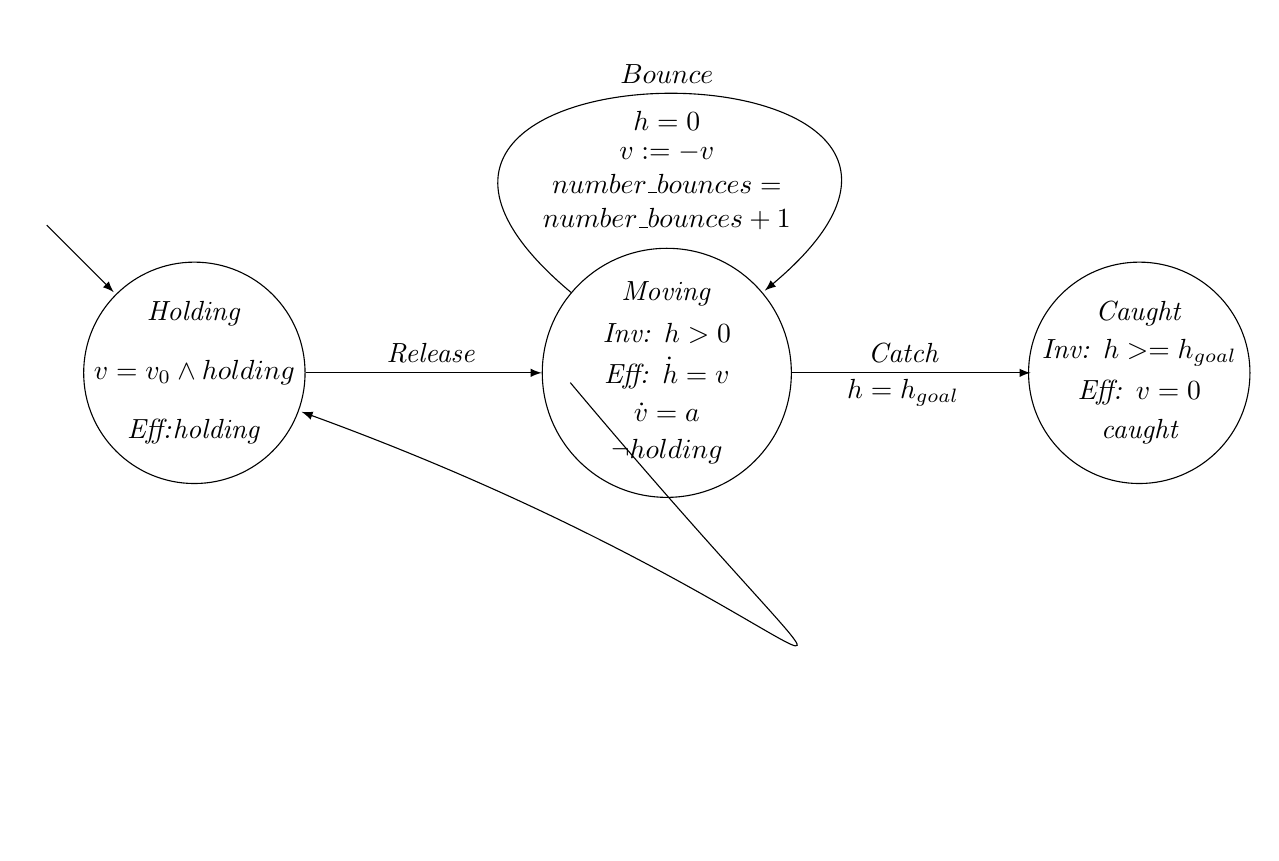
\begin{tikzpicture}[>=latex]
  \begin{scope}

%   \draw  (1,1) rectangle (7,1.5);

%\filldraw[black] (0,0) circle (2pt) node[anchor=west] {s};
\node (p1) at (-6,0.0) {};
\node (p2) at (-1.33,0.0) {};
\node (p3) at (4.745,0.0) {};




\node[circle, inner sep=4pt,draw, minimum height=80pt] (p1) at (-6,0) {};
\node (p4) at (-8,2.0) {};

\draw[->,shorten >=1pt] (p4) to  (p1);
\node (p0_d) at (-6.0,0.75) {\textit{Holding}};
%\node (p0_d) at (-6.0,0.25) {\textit{Inv:}   $h=h_0$};
\node (p0_d) at (-6.0,0){$v=v_0 \wedge holding $};
\node (p0_d) at (-6.0,-0.75) {\textit{Eff:}\textit{holding}};
\node (p0_d) at (-3.0,0.25) {$\textit{Release}$};
\draw[->,shorten >=1pt] (p2) to [out=310,in=340,loop,looseness=5.5] (p1);
\node (p0_d) at (-3.0,-0.25) {};

\node[circle, inner sep=4pt,draw, minimum height=90pt] (p2) at (0,0) {};
\draw[->] (p1) edge (p2);

\node (p1_d) at (0.0,1.0) {\textit{Moving}};
\node (p1_d) at (0.0,0.5) {\textit{Inv:} $h>0$};
\node (p1_d) at (0.0,0.0) {\textit{Eff:}  $\dot{h}=v$};
\node (p1_d) at (0.0,-0.5) {$\dot{v}=a$};
\node (p1_d) at (0.0,-1.0) {$\neg holding$};
\draw[->] (p2) edge (p3);
\node (p1_d) at (3.0,0.25) {$\textit{Catch}$};
\node (p1_d) at (3.0,-0.25) {$h=h_{goal}$};
\draw[->,shorten >=1pt] (p2) to [out=140,in=40,loop,looseness=5.5] (p2);
\node (p1_d) at (0.0, 3.2) {$h=0$};
\node (p1_d) at (0.0, 2.8) {$v:=-v$};
\node (p1_d) at (0.0, 2.4) {$number\_bounces = $};
\node (p1_d) at (0.0, 1.95) {$number\_bounces + 1 $};
\node (p1_d) at (0.0, 3.8) {$Bounce$};

\node[circle, inner sep=4pt,draw, minimum height=80pt] (p3) at (6,0) {};
\node (p2_d) at (6.0,0.75) {\textit{Caught}};
\node (p2_d) at (6.0,0.25) {\textit{Inv:}   $h>=h_{goal}$};
\node (p2_d) at (6.0,-0.25){\textit{Eff:}  $v=0$};
\node (p2_d) at (6.0,-0.75) {$\textit{caught}$};
\end{scope}
\end{tikzpicture}
\caption{Free Fall hybrid automaton}
\label{fig:Free Fall hybrid automaton}
\end{figure*}

Considering the dynamics of the problem, we have three discrete locations. The initial state which indicates our first discrete mode: the ball is held at the height $h_0$ and the velocity $v = v_0$ (this state is shown by the left circle in Figure~\ref{fig:Free Fall hybrid automaton}). As soon as the ball is released, a discrete transition moves the automaton to the next discrete location representing the moving state (this state is shown by the middle circle in Figure~\ref{fig:Free Fall hybrid automaton}). In this state, the height of the ball changes according to the velocity $\dot{h}=v$, and the velocity changes according to acceleration $\dot{v}=a$. As soon as the height of the ball becomes zero ($h=0$), the ball bounces. A discrete transition negates the velocity.

The robot can catch the ball as soon as the conditions of the goal state are satisfied. In Figure~\ref{fig:Free Fall hybrid automaton} this condition is that the ball is at a specific height $h=h_{goal}$. At this point, the hybrid automaton will move to the next discrete state which represents the state where the ball has been caught by the robot (this state is shown by the right circle in Figure~\ref{fig:Free Fall hybrid automaton}).

\subsection{PDDL+ Model of the Free Fall Problem}

In this section we describe how the hybrid automaton of the Free Fall problem can be written in PDDL+. A planning model represented in PDDL+ consists of the domain and the problem instance. The domain model lists the action schema and the possible processes and events. The problem instance describes the objects, the initial state, and the goal state. The domain corresponding to the hybrid automaton in Figure~\ref{fig:Free Fall hybrid automaton} is shown in Figure~\ref{fig:freefall domain}, while the problem instance is shown in Figure~\ref{fig:freefall problem}. In this problem we include a single ball, \textit{ball1}, and define that the robot should catch the ball when the height of the ball is 5.

\begin{figure*}[thb]
\small
\begin{BVerbatim}
(define (domain dropping_ball)
(:requirements :fluents :typing :durative-actions :time :negative-preconditions :duration-inequalities :timed-initial-literals) ;;:durative-actions :time :negative-preconditions :duration-inequalities

(:types ball)
(:predicates (holding ?b - ball) (caught ?b - ball))
(:functions
    (velocity ?b - ball)
    (height ?b - ball)
    (catch_height)
    (number_bounces ?b - ball)
    (catch_bounce)
)

(:action release
 :parameters (?b - ball)
 :precondition (and (holding ?b) (= (velocity ?b) 0))
 :effect (and (not (holding ?b)))
)

(:process moving
 :parameters (?b - ball)
 :precondition (and (not (holding ?b)) (>= (height ?b) 0))
 :effect (and
    (increase (velocity ?b) (* #t -9.8) )
    (increase (height ?b) (* #t (velocity ?b))))
 )
 
(:event bounce
 :parameters (?b - ball)
 :precondition (and (< (velocity ?b) 0) (<= (height ?b) 0.000001))
 :effect (and 
    (increase (number_bounces ?b) 1)
    (assign (velocity ?b) (* -1 (velocity ?b))))
)

(:action catch
 :parameters (?b - ball)
 :precondition (and
    (>= (height ?b) (catch_height))
    (<= (height ?b) (+ (catch_height) 0.1))
    (>= (number_bounces ?b) (catch_bounce)))
 :effect (and
    (holding ?b)
    (assign (velocity ?b) 0)
    (caught ?b)))
)

\end{BVerbatim}
\caption{Simplified PDDL+ domain description for Free Fall.}
\label{fig:freefall domain}
\end{figure*}

% working example problem (Free fall)
\begin{figure*}[thb]
\small
\centering
\begin{BVerbatim}
(define (problem dropping_ball_1)
(:domain dropping_ball)
(:objects ball1 - ball)

(:init 
    (holding ball1)
    (= (velocity ball1) 0)
    (= (height ball1) 10)
    (= (catch_height) 5)
    (= (number_bounces ball1) 0)
    (= (catch_bounce) 1)
)

(:goal
    (caught ball1)
))
\end{BVerbatim}
\caption{Simplified PDDL+ Free Fall problem file}
\label{fig:freefall problem}
\end{figure*}

Grounding the problem by applying the objects from the problem instance to the predicates of the domain forms the propositional variables $(holding\ ball1)$ and $(caught\ ball1)$. These variables describe a discrete state-space of 4 states:
\begin{itemize}
\item The initial state in which $(holding\ ball1)$ is true and $(caught\ ball1)$ corresponds to the \emph{Holding} location of the hybrid automaton.
\item The state in which both variables are false is reached after applying the action $(release\ ball1)$. This state corresponds to the \emph{Moving} location of the hybrid automaton. In this discrete state, the process $(moving\ ball1)$ asserts the continuous change on the numeric variables.
\item The state where both variables are true, is reached by applying the action $(catch\ ball1)$. This state corresponds to the \emph{Caught} location in the hybrid automaton. The goal holds in this state.
\item The state in which $(holding\ ball1)$ is false and $(caught\ ball1)$ is true is not reachable from the initial state without first reaching the goal, and does not appear in the hybrid automaton.
\end{itemize}

The continuous change of the location \emph{Moving} is asserted by the process $(moving\ ball1)$, which is active while its preconditions, $(not (holding\ ball1))$ and $(>= (height\ ball1)\ 0)$, are satisfied. The event $(bounce\ ball1)$ has no effect upon the discrete state, instead affecting only the numeric variables and also increases the $(number\_bounces)$. This event corresponds to the self-looping transition \emph{Bounce} in the hybrid automaton. As explained previously, an event is triggered as soon as its preconditions are satisfied. In this case, the event will be triggered as soon as the ball has reached the floor. This precondition is shown as $(<= \ (height \  ?b) \ 0.000001)$. Note that in the automaton, the transition \emph{Bounce} is a must transition, in the sense that is a must be triggered as soon as $h=0$ as this violates the invariant of \emph{Moving}. Similarly, events in PDDL+ follow a must semantics and are triggered as soon as their preconditions are satisfied. 
%The reason for modelling this precondition as an inequality less than or equal to a small constant is to get a valid plan using the validator~\cite{howey2004val}.
